En esta sección presentamos los resultados experimentales obtenidos para los dos problemas estudiados: \emph{ordenamiento de arreglos} y \emph{multiplicación de matrices}.

\paragraph{Reproducibilidad.}
Los datos de medición (tiempo y memoria) se guardan en la carpeta \texttt{data/measurements/} de cada módulo, y las salidas (arreglos o matrices) en \texttt{data/array\_output/} y \texttt{data/matrix\_output/}. 
Los gráficos se generan con el script \texttt{plot\_generator.py} y se almacenan en \texttt{data/plots/} dentro de cada módulo (\texttt{sorting} y \texttt{matrix\_multiplication}). % sin rutas largas para evitar overfull

\subsubsection*{Ordenamiento de arreglos}

\textbf{Tiempo.} En la Figura~\ref{fig:sorting} (izquierda) se observa que \texttt{std::sort} es sistemáticamente el más rápido en todo el rango de $n$, seguido de \texttt{MergeSort} y \texttt{QuickSort} (cuando alcanza a ejecutarse). La tendencia de estas tres curvas es coherente con $O(n\log n)$. \texttt{InsertionSort} exhibe el crecimiento cuadrático esperado, volviéndose impracticable para $n \ge 10^5$. \texttt{PandaSort} escala peor que los $O(n\log n)$, con tiempos sensiblemente mayores en tamaños grandes.

\textbf{Memoria.} En la Figura~\ref{fig:sorting} (derecha) se aprecia que \texttt{InsertionSort}, \texttt{QuickSort} y \texttt{std::sort} son casi \emph{in-place} (overhead adicional despreciable), mientras que \texttt{MergeSort} presenta el consumo lineal $O(n)$ que exige su arreglo auxiliar. \texttt{PandaSort} muestra un consumo notoriamente superior en $n$ grandes, consistente con su diseño con estructuras auxiliares adicionales.

\begin{figure}[H]
    \centering
    \begin{minipage}[t]{0.49\textwidth}
        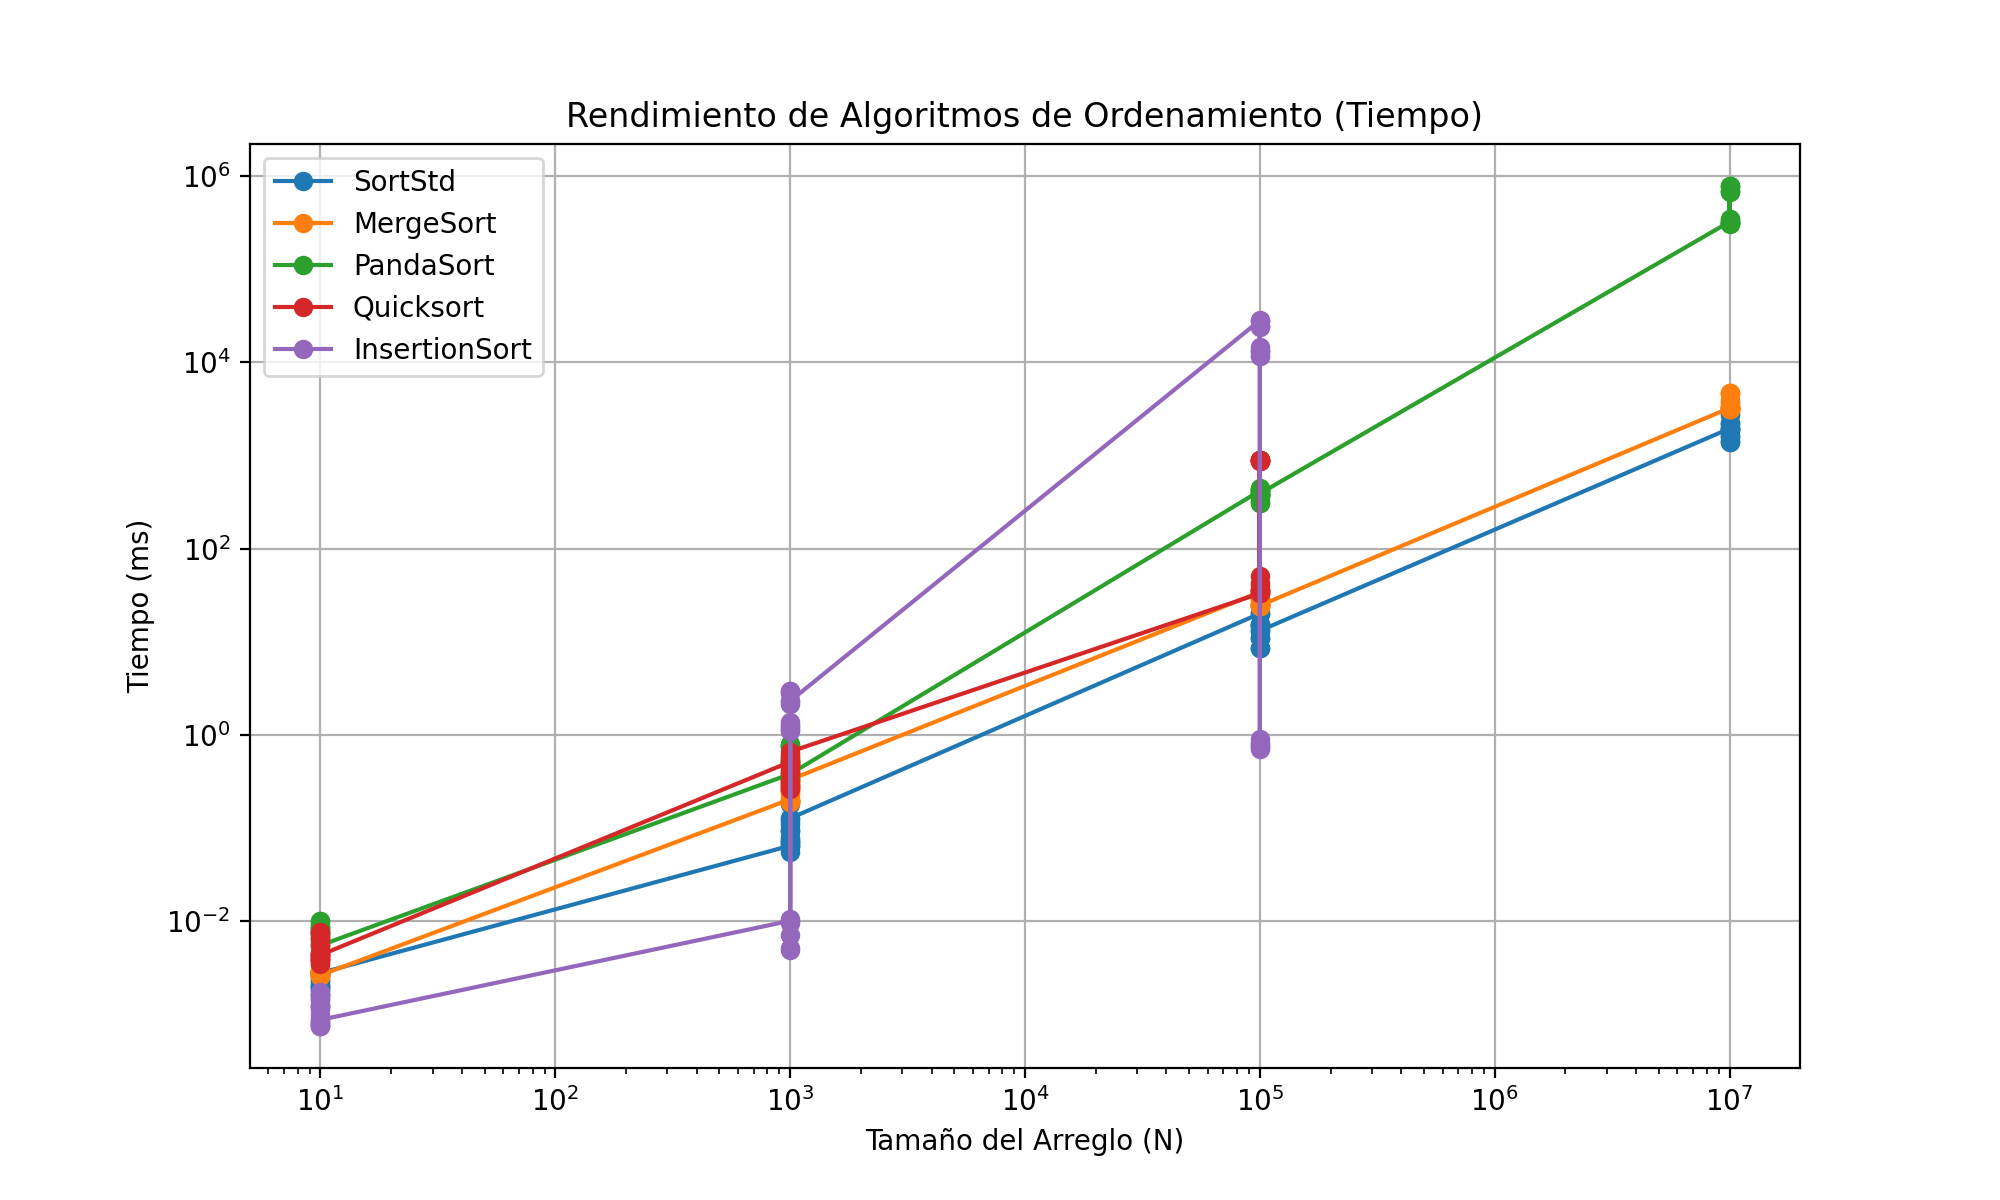
\includegraphics[width=\textwidth]{../code/sorting/data/plots/tiempo.png}
    \end{minipage}\hfill
    \begin{minipage}[t]{0.49\textwidth}
        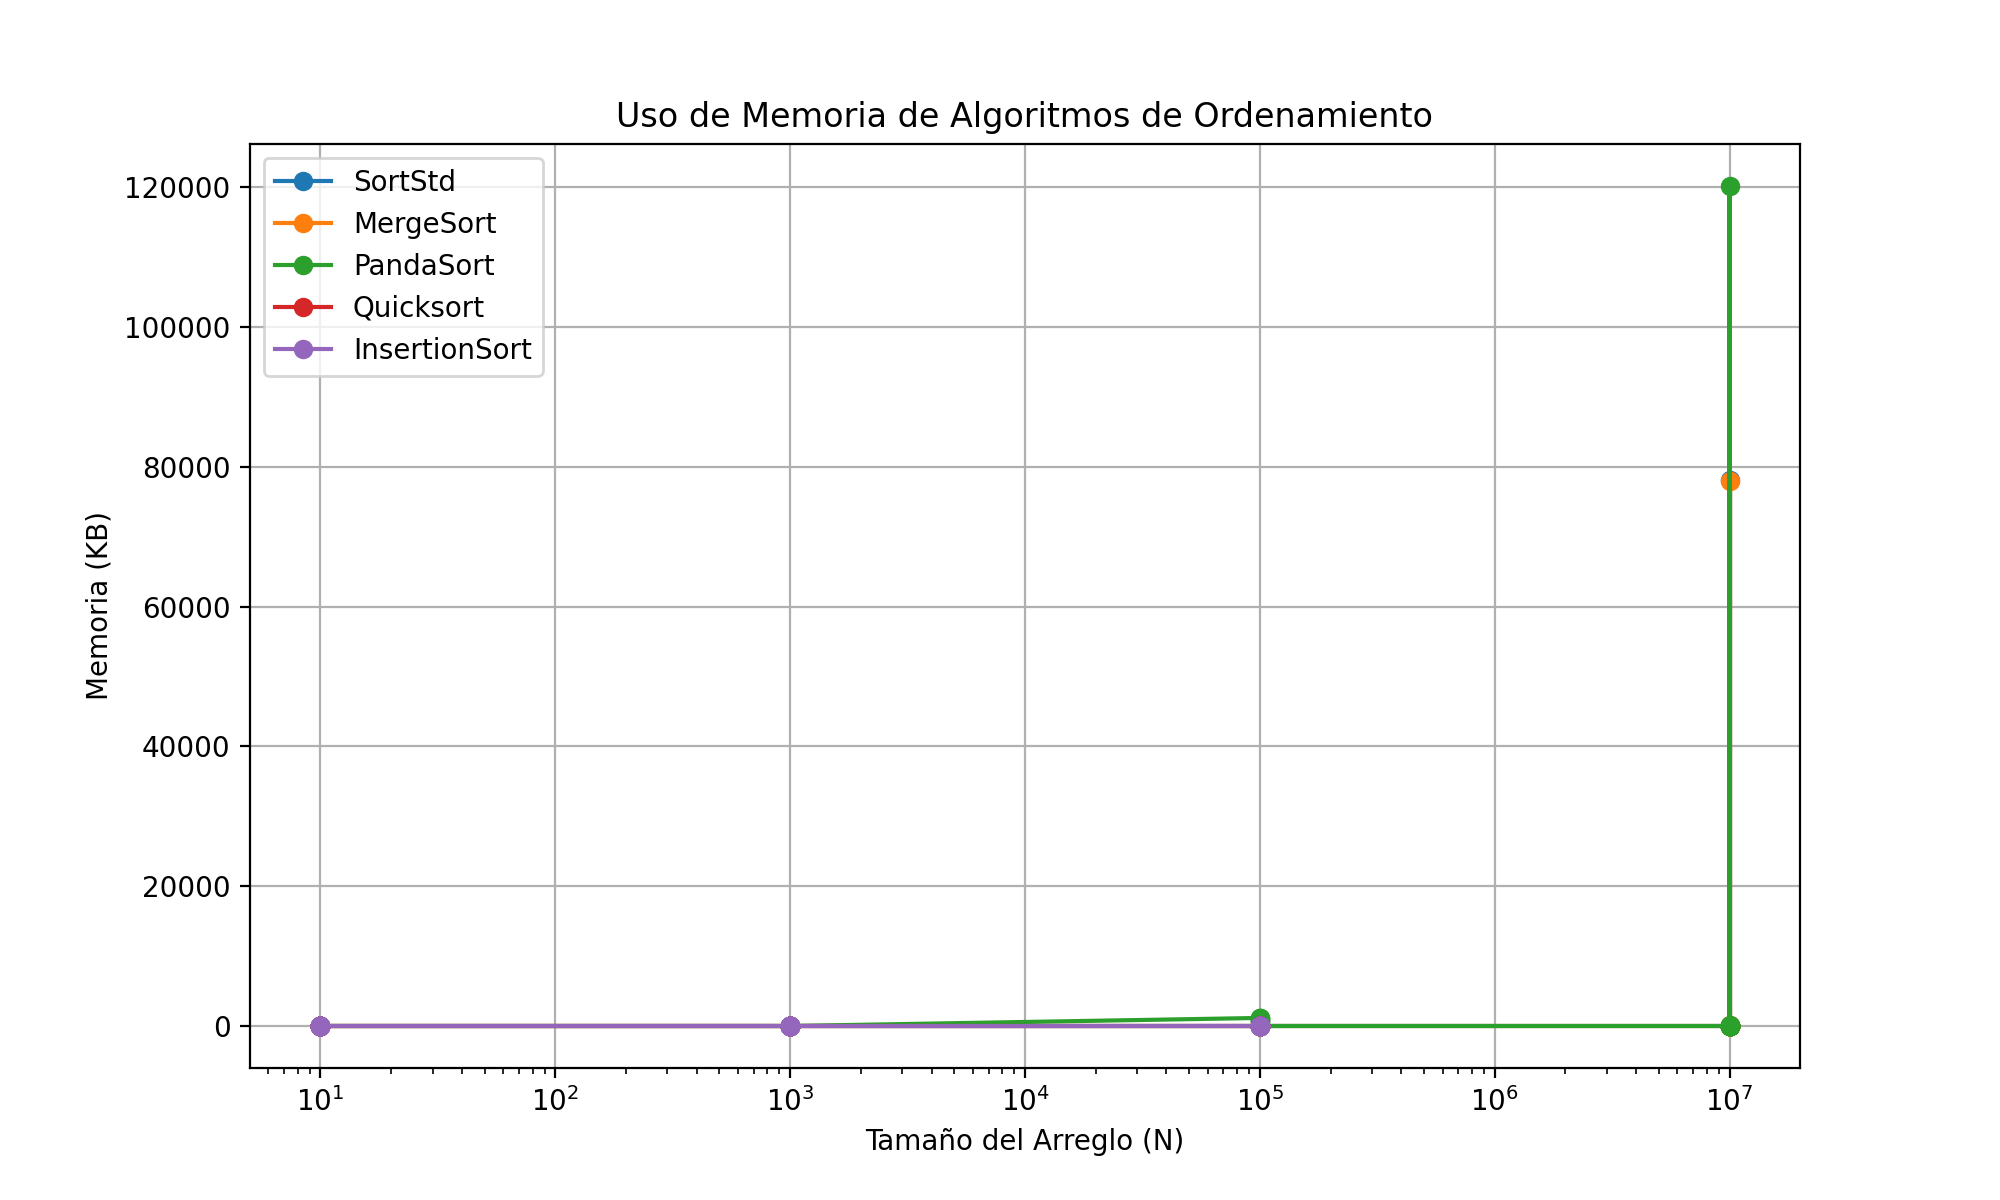
\includegraphics[width=\textwidth]{../code/sorting/data/plots/memoria.png}
    \end{minipage}
    \caption{Ordenamiento: (izq.) tiempo de ejecución vs. tamaño del arreglo; (der.) memoria adicional usada.}
    \label{fig:sorting}
\end{figure}

\subsubsection*{Multiplicación de matrices}

\textbf{Tiempo.} La Figura~\ref{fig:matmul} (izquierda) muestra que el método \texttt{Naive} resulta más rápido que \texttt{Strassen} en los tamaños evaluados (hasta $n=2^{10}$). Pese a la mejor complejidad asintótica de Strassen ($O(n^{\log_2 7}) \approx O(n^{2.81})$), en nuestra escala finita su \emph{overhead} domina: muchas sumas/restas de subbloques, llamadas recursivas y manejo de temporales elevan las constantes ocultas y penalizan la localidad de caché. Sin un umbral híbrido para conmutar a \texttt{Naive} en subproblemas pequeños, el punto de cruce donde Strassen superaría a \texttt{Naive} no se alcanza en esta infraestructura.

\textbf{Memoria.} En la Figura~\ref{fig:matmul} (derecha) \texttt{Strassen} utiliza más memoria que \texttt{Naive}. Aunque ambos conservan orden $O(n^2)$ en espacio, Strassen requiere temporales por nivel recursivo (sumas/restas y productos parciales), lo que incrementa la constante asociada al término cuadrático. Esto se refleja empíricamente en una brecha consistente a favor de \texttt{Naive}.

\begin{figure}[H]
    \centering
    \begin{minipage}[t]{0.49\textwidth}
        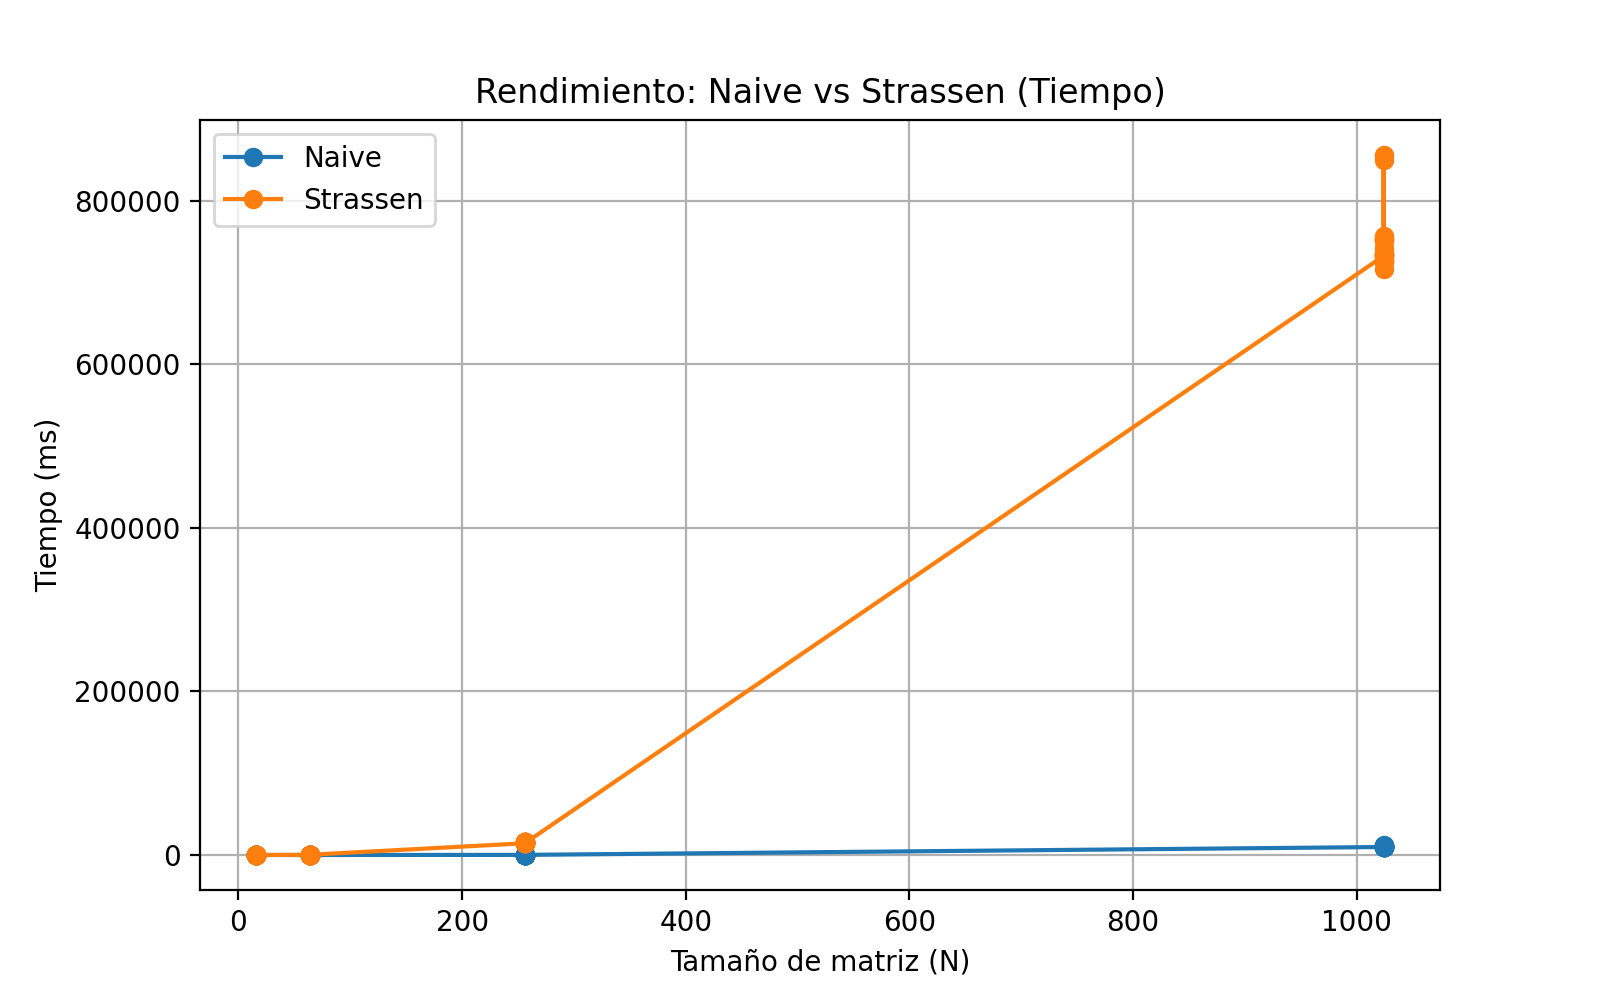
\includegraphics[width=\textwidth]{../code/matrix_multiplication/data/plots/tiempo.png}
    \end{minipage}\hfill
    \begin{minipage}[t]{0.49\textwidth}
        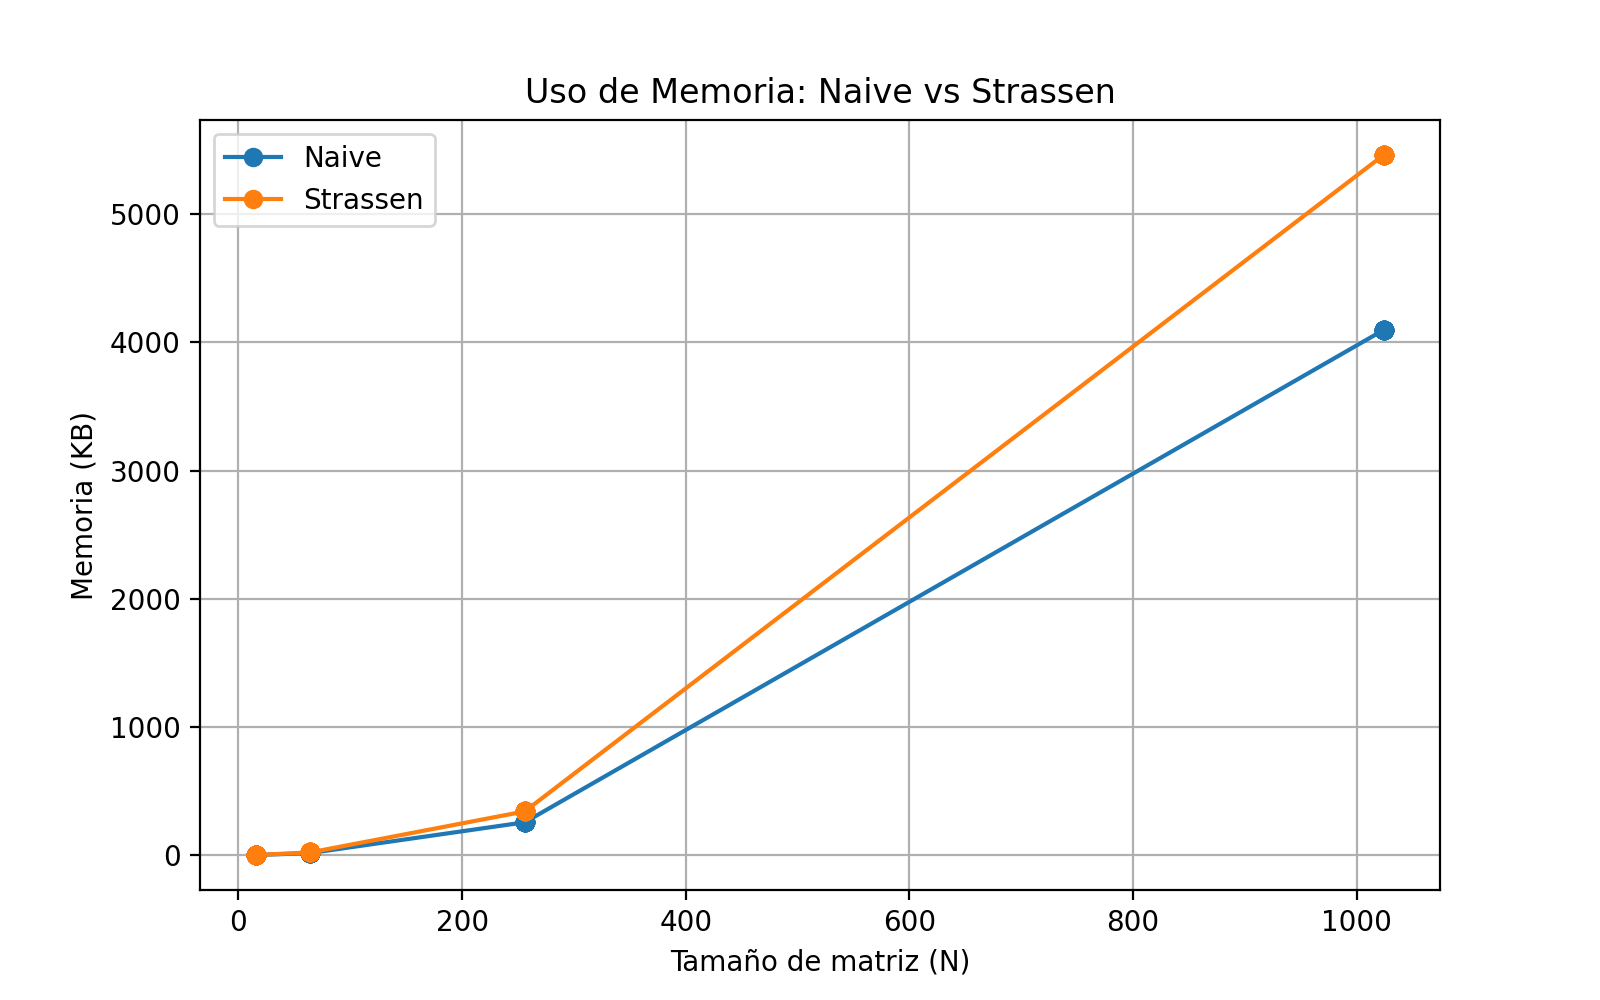
\includegraphics[width=\textwidth]{../code/matrix_multiplication/data/plots/memoria.png}
    \end{minipage}
    \caption{Multiplicación de matrices: (izq.) tiempo de ejecución; (der.) memoria adicional.}
    \label{fig:matmul}
\end{figure}